\section{Budget at completion}
\newcolumntype{L}[1]{>{\raggedright\let\newline\\\arraybackslash\hspace{0pt}}m{#1}}
\newcolumntype{C}[1]{>{\centering\let\newline\\\arraybackslash\hspace{0pt}}m{#1}}
\newcolumntype{R}[1]{>{\raggedleft\let\newline\\\arraybackslash\hspace{0pt}}m{#1}}

\begin{longtable}[H]{C{4cm}}
	\toprule[2pt]
	\textbf{Budget At Completion}\\
	\textbf{3.628.886\euro}\\
	\toprule[2pt]
\end{longtable}

Next, it is shown the budget at completion and its distribution according to the typology of the tasks to which it is destined. A distinction between four types of tasks is done: project management tasks, quality and administration tasks, development tasks and commercial tasks.
\begin{figure}[H]
	\centering
	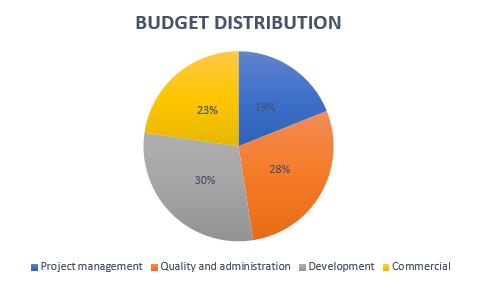
\includegraphics[width=0.8\linewidth]{./images/BudgetDistribution}
	\caption[Budget distribution]{Budget distribution.}
	\label{fig:BudgetDistribution}
\end{figure} 

\begin{longtable}[H]{L{5cm} R{2.5cm}}
	\toprule[2pt]
	\textbf{Task topology} & \textbf{Amount (\euro)}\\
	Project management& 687.369\\
	Quality and administration& 1.037.827\\
	Development & 1.078.622\\
	Commercial & 825.067\\
	\toprule[2pt]
\end{longtable}

Despite allocating most of the budget to the development of the product, it can be seen that the difference in the cost of other types of tasks is not very large. This shows once again that in a project the product itself is not everything, but it is necessary to cover expenses of all kinds that are not related to the technical part. 